\chapter{Présentation du langage R}
\label{chap:presentation}

\section{Bref historique}
\label{sec:presentation:historique}

À l'origine fut le S, un langage pour «programmer avec des données»
développé chez Bell Laboratories à partir du milieu des années 1970
par une équipe de chercheurs menée par John~M.\ Chambers. Au fil du
temps, le S a connu quatre principales versions communément
identifiées par la couleur du livre dans lequel elles étaient
présentées: %
version «originale», %
version 2, %
version 3 et %
version 4; %
voir aussi <citation> et <citation> pour plus de détails.

Dès la fin des années 1980 et pendant près de vingt ans, le S a
principalement été popularisé par une mise en {\oe}uvre commerciale
nommée S-PLUS. En 2008, Lucent Technologies a vendu le langage S à
Insightful Corporation, ce qui a effectivement stoppé le développement
du langage par ses auteurs originaux. Aujourd'hui, le S est
commercialisé de manière relativement confidentielle sous le nom
Spotfire S$+$ par TIBCO Software.

Ce qui a fortement contribué à la perte d'influence de S-PLUS, c'est
une nouvelle mise en {\oe}uvre du langage développée au milieu des
années 1990. Inspirés à la fois par le S et par Scheme (un dérivé du
Lisp), Ross Ihaka et Robert Gentleman proposent un langage pour
l'analyse de données et les graphiques qu'ils nomment R. À la
suggestion de Martin Maechler de l'ETH de Zurich, les auteurs décident
d'intégrer leur nouveau langage au projet GNU\footnote{%
  \url{http://www.gnu.org}}, %
faisant de R un logiciel libre.

Ainsi disponible gratuitement et ouvert aux contributions de tous,
R gagne rapidement en popularité là même où S-PLUS avait acquis ses
lettres de noblesse, soit dans les milieux académiques. De simple
dérivé «\emph{not unlike S}», R devient un concurrent sérieux à
S-PLUS, puis le surpasse lorsque les efforts de développement se
rangent massivement derrière le projet libre. D'ailleurs John Chambers
place aujourd'hui ses efforts de réflexion et de développement dans le
projet R.


\section{Interfaces}
\label{sec:presentation:interfaces}

R est d'abord et avant tout une application n'offrant qu'une invite de
commande du type de celle présentée à la
\ref{fig:presentation:console}. En soi, cela n'est pas si différent
d'un tableur tel que Excel: la zone d'entrée de texte dans une cellule
n'est rien d'autre qu'une invite de commande\footnote{%
  Merci à Markus Gesmann pour cette observation.}, par ailleurs aux
capacités d'édition plutôt réduites.

\begin{figure}
  \centering
%  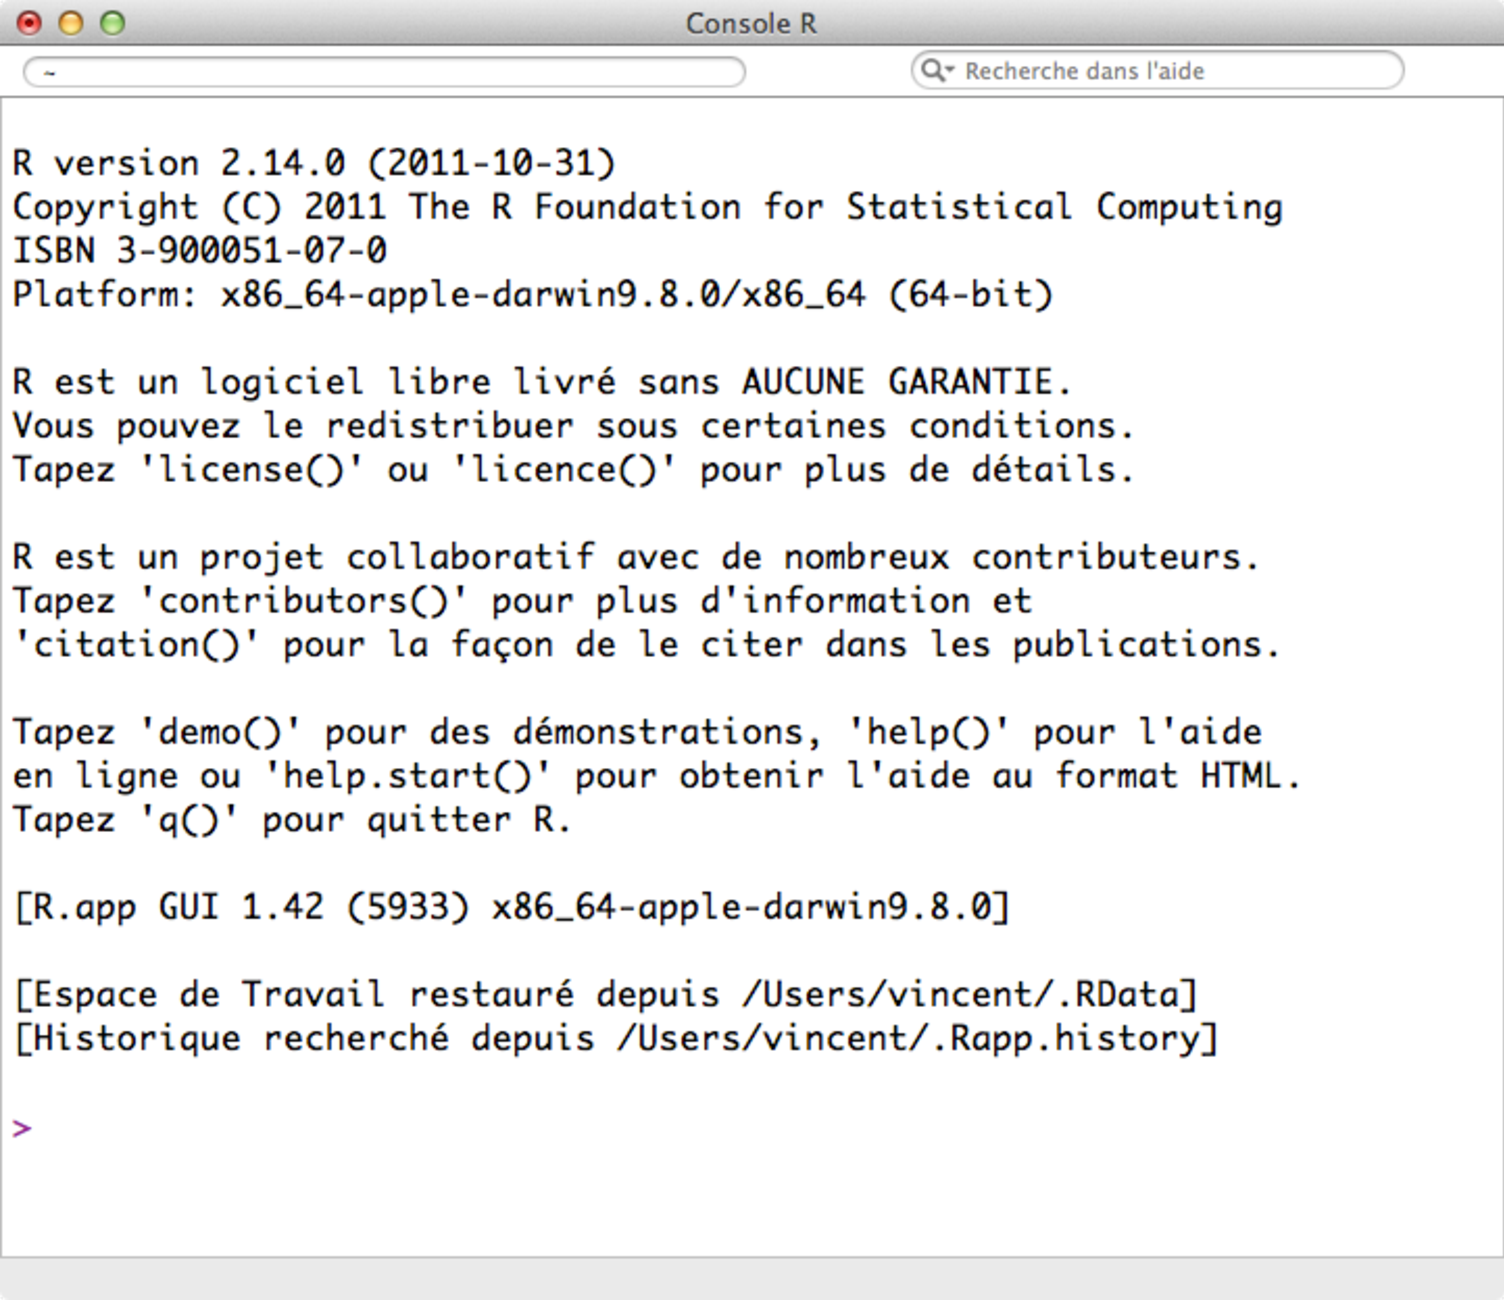
\includegraphics[width=\textwidth]{console-screenshot}
  \caption{Fenêtre de la console sous Mac OS~X au démarrage de R}
  \label{fig:presentation:console}
\end{figure}

\begin{itemize}
\item Sous Unix et Linux, R n'est accessible que depuis la ligne de
  commande du système d'exploitation (terminal). Aucune interface
  graphique n'est offerte avec la distribution de base de R.
\item Sous Windows, une interface graphique plutôt rudimentaire est
  disponible. Elle facilite certaines opérations tel que
  l'installation de packages externes, mais elle offre autrement peu
  de fonctionnalités additionnelles pour l'édition de code R.
\item L'interface graphique de R sous Mac OS~X est la plus élaborée.
  Outre la console présentée à la
  \ref{fig:presentation:console}, l'application \texttt{R.app}
  comporte de nombreuses fonctionnalités, dont un éditeur de code
  assez complet.
\end{itemize}
